\chapter{Related work} \label{ch:related_work}
In this chapter, we present studies in the field of code clone refactoring. The sections are ordered chronologically, because many of these studies use findings of preceding studies.

\section{SUPREMO}
A thesis by Golomingi~\cite{koni2001scenario} is the first to explore mapping the relation between clone instances to refactoring methods. The author analyses the refactoring methods described by Martin Fowler \cite{fowler1999refactoring}. Mapping these to relations between clones results in Table \ref{tab:relationrefactoring}.

\begin{table}[H]
\centering
\resizebox{\textwidth}{!}{%
\begin{tabular}{lcccccccc}
\toprule
                     & Ancestor   & \begin{tabular}[c]{@{}l@{}}Common\\ Hierarchy\end{tabular} & \begin{tabular}[c]{@{}l@{}}First\\ Cousin\end{tabular} & \begin{tabular}[c]{@{}l@{}}Same\\ Method\end{tabular} & Sibling    & \begin{tabular}[c]{@{}l@{}}Single\\ Class\end{tabular} & Superclass & Unrelated \\ \midrule
Extract Method       & \checkmark & \checkmark                                                 & \checkmark                                             & \checkmark                                            & \checkmark & \checkmark                                             &            &           \\
Insert Method Call   &            &                                                            &                                                        & \checkmark                                            &            & \checkmark                                             &            &           \\
Insert Super Call    &            &                                                            &                                                        &                                                       &            &                                                        & \checkmark &           \\
Parameterization     & \checkmark & \checkmark                                                 & \checkmark                                             & \checkmark                                            & \checkmark & \checkmark                                             & \checkmark &           \\
Pull Up Method       & \checkmark & \checkmark                                                 & \checkmark                                             &                                                       & \checkmark &                                                        & \checkmark &           \\
Form Template Method & \checkmark & \checkmark                                                 & \checkmark                                             & \checkmark                                            & \checkmark & \checkmark                                             & \checkmark &           \\
Push Down Method     &            &                                                            &                                                        &                                                       &            &                                                        & \checkmark &           \\
Extract Superclass   &            & \checkmark                                                 & \checkmark                                             &                                                       & \checkmark &                                                        &            &           \\ \bottomrule
\end{tabular}%
}
\caption{Mapping clone relations to refactoring techniques \cite{koni2001scenario}}
\label{tab:relationrefactoring}
\end{table}

The author then proposes a tool named ``SUPREMO''. This tool determines the relations between clone instances, computes the impact of the clones on system design and proposes refactorings. It also features visualizations to show how clones are related in the inheritance structure. SUPREMO is written for the Smalltalk programming language. The authors verify their approach by presenting several cases in which their tool analyses source code and outputs a refactoring suggestion. In our work, we use these same relations and refactoring techniques.

\section{Aries}
A study by Higo et al.~\cite{higo2004aries, higo2008metric} looks into to what extent clones can be refactored. The authors look into what parts of a clone can be extracted to a new method. They define that partially cloned blocks obstruct method extraction. They propose to make the clone smaller to find a part of the clone that can be refactored. This is similar to our ``partial block'' category of Section~\ref{sec:refactorabilitysetup} and our discussion in Section~\ref{sec:partialblockdiscussion}.

Higo et al. also look into the amount of variability that can be allowed between clone fragments. Figure~\ref{fig:higomerge} shows an example of merging two code fragments from this study. In this figure, the clone spans a part of a different block so it cannot be refactored. They propose to omit both ``else if'' lines from the merged fragment so that it can be refactored (in our study we would have flagged these clones as ``partial block'' and thus unsuitable for refactoring). They also allow variability in literals and variables and replace them with method parameters.

\begin{figure}[H]
  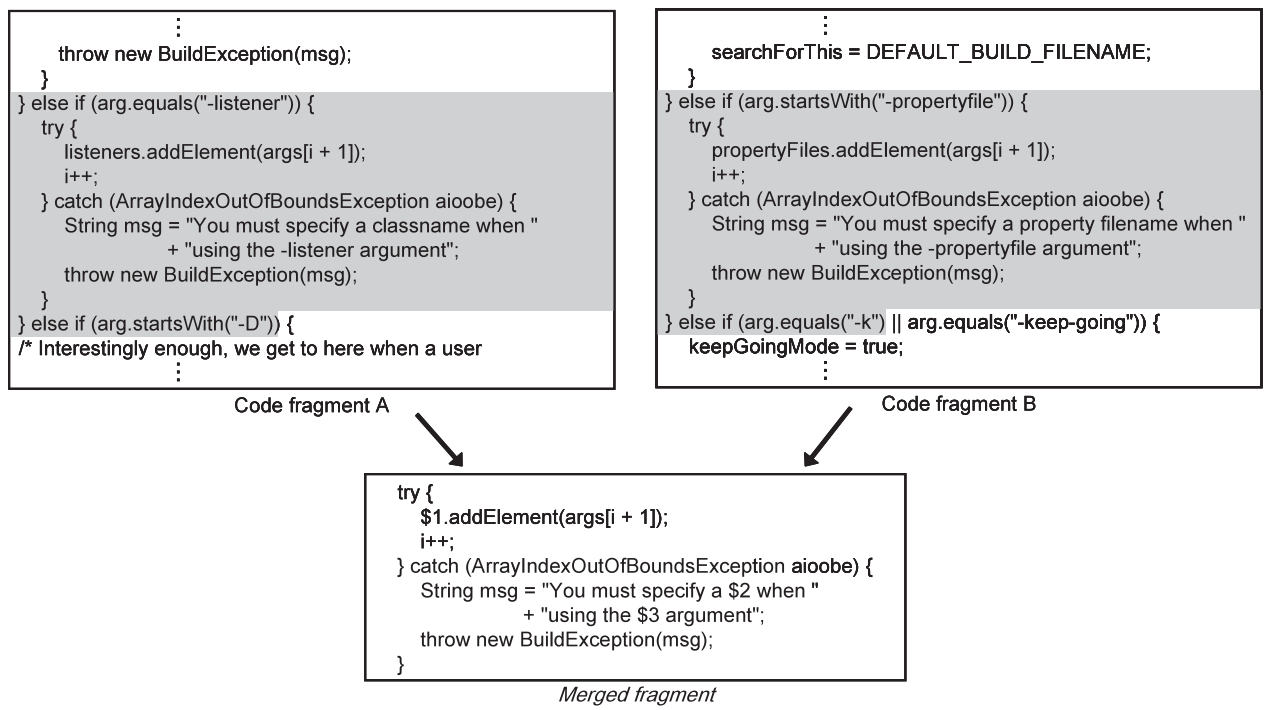
\includegraphics[width=1\textwidth]{img/higo}
  \caption{Example of merging two code fragments from Higo et al.~\cite{higo2008metric}.}
  \label{fig:higomerge}
\end{figure}

Higo et al. propose a tool named Aries~\cite{higo2004aries, higo2008metric} that focuses on the detection of refactorable clones. They focus entirely on whether a clone \textbf{can} be refactored and not whether it \textbf{should} be refactored. This tool only proposes refactoring opportunities and does not provide help in the process of applying the refactoring, which our work does.

\section{Duplicated Code Refactoring Advisor (DCRA)}
Fontana et al.~\cite{fontana2012duplicated, fontana2015duplicated} combine the research by Golomingi~\cite{koni2001scenario} with clone types 1 and 3 \cite{roy2007survey}. They use a large corpus~\cite{tempero2010qualitas} on which they perform statistical analyses of clone relations together with clone types. Table \ref{tab:dcra-relation} displays the result of this analysis. We added percentages and ordering to this table for easier comparison with the results of our work (see \ref{sec:relationresults}). We also added the percentages of our work to this table.

\begin{table}[H]
\centering
\begin{tabular}{@{}lrrrrr@{}}
\toprule
                         & Type 1 & Percentage & Type 3 & Percentage & Type 1R (Our Work) \\ \midrule
Same Class               & 5,645  & 32.1\%     & 51,308 & 28.7\% & 26.8\%    \\
Same External Superclass & 4,384  & 25.0\%     & 66,391 & 37.1\% & 20.6\%   \\
Unrelated Class          & 2,758  & 15.7\%     & 35,035 & 19.6\% & 18.4\%    \\
Sibling Class            & 2,721  & 15.5\%     & 13,868 & 7.8\%  & 18.2\%    \\
Common Hierarchy Class   & 970    & 5.5\%      & 3,152  & 1.8\%  & 0.8\%    \\
Same Method              & 569    & 3.2\%      & 4,901  & 2.7\%  & 10.5\%    \\
First Cousin Class       & 416    & 2.4\%      & 2,980  & 1.7\%  & 1.4\%    \\
Superclass               & 91     & 0.5\%      & 981    & 0.5\%  & 3.1\%    \\
Ancestor Class           & 13     & 0.1\%      & 281    & 0.2\%  & 0.2\%    \\ \bottomrule
\end{tabular}
\caption{Clone relation analysis by Fontana et al. \cite{fontana2012duplicated} for type 1 and 3 clones measured over the Qualitas Corpus \cite{tempero2010qualitas}.}
\label{tab:dcra-relation}
\end{table}

Some of our results differ quite a lot from their results. We think this is mostly accounted due to two differences in their setup:
\begin{itemize}
\item The used clone type definitions differ (type 1 vs type 1R).
\item Fontana et al. use a corpus consisting of large higher-quality open-source software systems \cite{tempero2010qualitas} where we use a more varied corpus \cite{githubCorpus2013}.
\item Fontana et al. use clone pairs while we use clone classes.
\end{itemize}

Fontana et al.~\cite{fontana2012duplicated, fontana2015duplicated} propose DCRA, a tool to suggest refactorings for the clones found by the NiCAD tool \cite{roy2008nicad, cordy2011nicad}. DCRA suggests refactorings to clones found in Java projects based on the mapping between relation and refactoring techniques shown in Table~\ref{tab:relationrefactoring}.

\section{JDeodorant} \label{sec:jdeodorant}
The most used clone refactoring tool is JDeodorant \cite{mazinanian2016jdeodorant}. This tool is based on a set of studies, that look into several aspects of the clone refactoring process. The first of these studies is ``Refactoring Clones: An Optimization Problem'' by Krishnan et al.~\cite{krishnan2013refactoring}. The authors describe clones that are refactored by extracting their functionality to a single method. They describe that variability between identifiers and literals have to become parameters in the extracted method. They identify the optimization problem where the variability between cloned fragments should be limited, to avoid limiting the reusability of methods because of too many method parameters. They propose an algorithm that calculates the variance between code fragments on basis of the difference in AST nodes.

In the second study, ``Unification and Refactoring of Clones'' by Krishnan et al.~\cite{krishnan2014unification}, the authors address the problem of the modifications made to copied fragments and their impact on the refactoring process. They identify a list of expressions in which they have found variability, which is displayed in Table~\ref{tab:krishnanvariability}. The authors map the variability in this table to refactoring opportunities. They list a set of four preconditions for the refactoring process:
\begin{enumerate}
  \item The parameterization of differences between the matched statements should not break existing data-, anti-, and output-dependences.
  \item The unmatched statements should be movable before or after the matched statements without breaking existing data-, anti-, and output-dependences.
  \item The duplicated code fragments should return at most one variable of the same type.
  \item Matched branching (\texttt{break}, \texttt{continue}) statements should be accompanied with corresponding matched loop statements.
\end{enumerate}
In our study, we address precondition 1 and 2 and propose a solution. To address precondition 1, we only refactor variability in such a way that existing data-, anti-, and output-dependences are not affected (see Section \ref{sec:type2r}). For precondition 2, we propose using conditional or lambda expressions to wrap the difference in statements (see Section \ref{sec:type3r}). For precondition 3 and 4, we flag these clones as ``not refactorable'' (see Section \ref{sec:refactorabilitysetup}).

\begin{table}[H]
\centering
\begin{tabular}{@{}lcc@{}}
\toprule
\textit{\textbf{Difference Type}} & \multicolumn{2}{c}{\textit{\textbf{Example}}}                                                \\ \midrule
Variable Identifier               & \multicolumn{1}{c|}{\texttt{int x = \textbf{y};}}       & \texttt{int x = \textbf{z};}       \\
Literal Value                     & \multicolumn{1}{c|}{\texttt{String s = \textbf{"s1"};}} & \texttt{String s = \textbf{"s2"};} \\
Method Name                       & \multicolumn{1}{c|}{\texttt{expr.\textbf{foo}(arg);}}   & \texttt{expr.\textbf{bar}(arg);}   \\
Argument Number                   & \multicolumn{1}{c|}{\texttt{foo(\textbf{arg0, arg1});}} & \texttt{foo(\textbf{arg0});}       \\
Caller Expression                 & \multicolumn{1}{c|}{\texttt{\textbf{expr.}foo(arg);}}   & \texttt{foo(arg);}                 \\
Array Dimension                   & \multicolumn{1}{c|}{\texttt{int x = a\textbf{[i]};}}    & \texttt{int x = a\textbf{[i][j]};} \\
AST Compatible                    & \multicolumn{1}{c|}{\texttt{int x = \textbf{foo()};}}   & \texttt{int x = \textbf{5};}       \\ \midrule
Operator                          & \multicolumn{1}{c|}{\texttt{int x = y \textbf{+} z;}}   & \texttt{int x = y \textbf{-} z;}   \\
Variable Type                     & \multicolumn{1}{c|}{\texttt{\textbf{int} x = 5;}}       & \texttt{\textbf{double} x = 5;}    \\ \bottomrule
\end{tabular}
\caption{Expression variability table from Krishnan et al.~\cite{krishnan2014unification}}
\label{tab:krishnanvariability}
\end{table}

A study by Tsantalis et al.~\cite{tsantalis2015assessing} looks into the refactorability of code clones. This results in a set of eight preconditions to determine whether a cloned fragment is refactorable. Four of these preconditions are similar to the Krishnan et al.~\cite{krishnan2014unification} study. The following preconditions have been added:
\begin{enumerate}
  \setcounter{enumi}{4}
  %\item The parameterization of the differences between the mapped statements should not break any existing control, data, anti, and output dependencies.
  \item Matched variables having different subclass types should call only methods that are declared in the common superclass or are being overridden in the respective subclasses.
  \item The parameterization of fields belonging to differences between the mapped statements is possible only if they are not modified.
  \item The parameterization of method calls belonging to differences between the mapped statements is possible only if they do not return a void type.
  %\item The unmapped statements should be movable before or after the mapped statements without breaking existing control, data, anti, and output dependencies.
  %\item The mapped statements within the clone fragments should return at most one variable of the same type to the original methods from which they are extracted.
  \item The mapped statements within the clone fragments should not contain any conditional return statements.
  %\item The mapped branching statements (break, continue) should be accompanied with the corresponding mapped loop statements
\end{enumerate}
In our study, we simplify precondition 5 by not allowing variability in types, because of which we satisfy this precondition. We address precondition 6 by allowing modified statements as return values (and turning the calls to the extracted method into variable assignments). If more than 1 variable is assigned or other return values would be present, we flag the cloned fragments as ``multiple return values'' (see Section~\ref{sec:refactorabilitysetup}). We address precondition 7 by using lambda expressions, which allow methods without return value to be used as parameters (using the \texttt{Runnable} interface). We address precondition 8 by analyzing all branches in the code. If all branches return, the fragment can still be refactored even though there is a conditional return statement.

After these studies that determine what preconditions apply to be able to refactor modified clones, the authors propose a tool named JDeodorant that helps in the process of refactoring such clones~\cite{mazinanian2016jdeodorant}. This tool takes the output of many popular clone detection tools \cite{kamiya2002ccfinder, deissenboeck2010flexible, jiang2007deckard, cordy2011nicad} and proposes refactoring opportunities. The tool is integrated in the Eclipse IDE, making it easier to directly apply the refactoring. The tool is based on previously discussed preconditions and does not allow refactorings if the preconditions are not met.

A study by Tsantalis et al.~\cite{tsantalis2017clone} looks into how lambda expressions can be used to help in the process of refactoring clones. They do this in order to mitigate some of the earlier established preconditions. Working with lambda expressions makes it possible to refactor statement gaps and expression differences. They find that lambda expressions are very suitable to refactor clones with variability. The authors do not discuss the impact of such refactorings on system maintainability, their main focus is to positively influence the refactorability of clone classes.

\section{Refactoring Technique for Large Groups of Software Clones}
In a thesis by AlWaqfi~\cite{alwaqfi2017refactoring} the author proposes a method for assessing refactorability of clone classes, whereas most of the previous tools only focus on clone pairs. The author surveys a set of clone detection tools \cite{kamiya2002ccfinder, baxter1999clonedr, jiang2007deckard, cordy2011nicad} and uses a publicly available dataset \cite{tsantalis2015assessing} to measure the amount of clones found by these tools. The resulting data shows that there is a lot of variability in the amount of detected clones between different clone detection tools. The author measures of how many clone instances there are in clone classes. According to these experiments, about 68\% of clone classes consist of 2 clone instances, 13\% have 3 clone instances, 7\% have 4 clone instances and about 12\% is even larger.

The authors perform a lot of statistical comparisons between clone detection tools. The part most relevant to our study is their measurements regarding refactorability. They find that about 29-54\% of clones are refactorable in the set of projects they inspect (Table 6.13 of \cite{alwaqfi2017refactoring}). To determine whether a clone is refactorable, the author uses the set of eight preconditions proposed by Tsantalis et al.~\cite{tsantalis2015assessing}.

\section{Pattern‐based clone Refactoring Inspection (PRI)}
A study by Chen et al.~\cite{chen2018clone} addresses the problem that developers cannot easily determine which clones can be refactored or how they should be maintained scattered throughout a large code base in evolving systems. They propose PRI, a technique for managing refactorings for clones with a Sibling relation. PRI is a plugin for the Eclipse IDE that shows which refactoring techniques can be used to refactor clones. Because it is integrated in the Eclipse IDE, the refactorings can be executed largely automatically, as this IDE has a large set of tools for performing such transformations.

Another feature of the PRI tool is to find incompletely refactored clones. To do this, PRI traces clones through revisions of a software project. When a clone class is incompletely refactored, PRI informs the user that there are clone instances for which an extracted method has already been created.

\section{Impact of Clone Refactoring on External Quality Attributes}
A study by Vashisht et al.~\cite{vashisht2018impact} determines the impact of clone refactoring on several quality attributes. They calculate the metrics of the system before refactoring, detect clones using CCFinder \cite{kamiya2002ccfinder}, use JDeodorant to refactor a subset of the detected clones \cite{mazinanian2016jdeodorant} and measure the metrics again after refactoring to assess the impact of the refactoring process on quality attributes. They conclude that clone refactoring affects some quality attributes positively and some negatively.

In this study, the authors only compare before- and after-snapshots of refactoring the entire system. This makes it hard to determine why some metrics are negatively influenced. In our study, we consider each separate refactoring, which yields more precise results.

\section{Clone Recommendation System for Extract Method Refactoring}
Yoshida et al.~\cite{yoshida2019proactive} propose a plugin for the Eclipse IDE that recommends clone refactoring candidates on basis of keystroke tracking. Whenever the user performs the ``Extract Method'' refactoring, the proposed system scans the project for clones that can now use the extracted method. It then shows the developer all places that should be refactored aswell now that a new method has been created. The approach was validated by requesting human participants to apply refactorings to open source systems. On average, it took participants 1,043 seconds to refactor 2.75 clones. They report that this is 35\% faster than when working with a popular clone detection tool (GemX).

\section{Effect of clone refactoring on the size of unit test cases}
Badri et al.~\cite{badri2019measuring} measure the impact on clone refactoring on metrics that affect the testability of software. The metrics they measure are size, cyclomatic complexity and coupling. To collect this data, they use two systems that have been de-duplicated manually. They conclude that there is a strong, positive correlation between clone refactoring and the reduction of the size of unit tests. They also show that code quality attributes that are related to testability are significantly improved.
